\begin{enumerate}[label=\thechapter.\arabic*,ref=\thechapter.\theenumi]

\item An $8$ bit ADC converts analog voltage in the range of $0$ to $+5\, V$ to the corresponding digital code as per the conversion characteristics shown in figure. For $V_{in} = 1.9922\, V$, which of the following digital output, given in hex, is true?

\begin{figure}[!h]
    \centering
    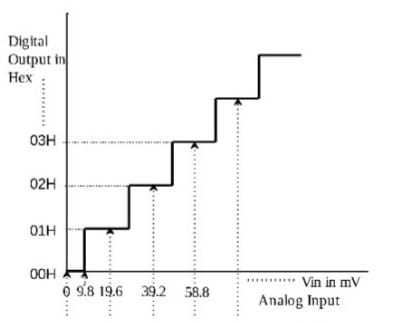
\includegraphics[width=\columnwidth]{2023/EE/40/figs/fig1.jpeg}
    \caption{}
    \label{fig:ADC_gate.ee.23.40}
\end{figure}
\begin{enumerate}[label=(\alph*)]
    \item $64H$
    \item $65H$
    \item $66H$
    \item $67H$
\end{enumerate} \hfill(GATE EE 40)

\solution
\iffalse
\let\negmedspace\undefined
\let\negthickspace\undefined
\documentclass[journal,12pt,twocolumn]{IEEEtran}
\usepackage{cite}
\usepackage{amsmath,amssymb,amsfonts,amsthm}
\usepackage{algorithmic}
\usepackage{graphicx}
\usepackage{textcomp}
\usepackage{xcolor}
\usepackage{txfonts}
\usepackage{listings}
\usepackage{enumitem}
\usepackage{mathtools}
\usepackage{gensymb}
\usepackage{comment}
\usepackage[breaklinks=true]{hyperref}
\usepackage{tkz-euclide} 
\usepackage{listings}
\usepackage{gvv}                                        
\def\inputGnumericTable{}                                
\usepackage[latin1]{inputenc}                            
\usepackage{color}                                       
\usepackage{array}                                       
\usepackage{longtable}                                   
\usepackage{calc}                              
\usepackage{tikz}
\usepackage{multirow}                                    
\usepackage{hhline}                                      
\usepackage{ifthen}                            
\usepackage{caption}
\usepackage{lscape}
\usepackage{amsmath}
\newtheorem{theorem}{Theorem}[section]
\newtheorem{problem}{Problem}
\newtheorem{proposition}{Proposition}[section]
\newtheorem{lemma}{Lemma}[section]
\newtheorem{corollary}[theorem]{Corollary}
\newtheorem{example}{Example}[section]
\newtheorem{definition}[problem]{Definition}
\newcommand{\BEQA}{\begin{eqnarray}}
\newcommand{\EEQA}{\end{eqnarray}}
\newcommand{\define}{\stackrel{\triangle}{=}}
\theoremstyle{remark}
\newtheorem{rem}{Remark}

\begin{document}

\bibliographystyle{IEEEtran}
\vspace{3cm}

\title{NCERT Math 11.9.2 Q8}
\author{EE23BTECH11009 - AROSHISH PRADHAN$^{*}$% <-this % stops a space
}
\maketitle
\newpage
\bigskip
\textbf{Question:} An $8$ bit ADC converts analog voltage in the range of $0$ to $+5\, V$ to the corresponding digital code as per the conversion characteristics shown in figure. For $V_{in} = 1.9922\, V$, which of the following digital output, given in hex, is true?

\begin{figure}[!h]
    \centering
    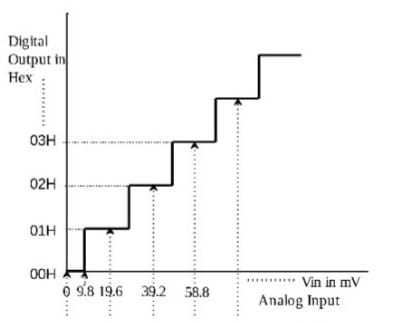
\includegraphics[width=\columnwidth]{2023/EE/40/figs/fig1.jpeg}
    \caption{}
    \label{fig:ADC_gate.ee.23.40}
\end{figure}
\begin{enumerate}[label=(\alph*)]
    \item $64H$
    \item $65H$
    \item $66H$
    \item $67H$
\end{enumerate}

\solution
\fi
\begin{table}[!h]
    \centering
    \resizebox{\columnwidth}{!}{\begin{tabular}{|c|c|c|}
    \hline
       \textbf{Symbol}  & \textbf{Value} & \textbf{Description}\\
    \hline
        $n$  &  $8$ &  Number of bits of ADC\\
    \hline
        $V_{min}$ & $0V$ & Minimum Analog Voltage\\
    \hline
        $V_{max}$ & $5V$ & Maximum Analog Voltage\\
    \hline
        $V_{in}$ & $1.9922 V$ & Input Voltage\\
    \hline
        $V_{out}$ & & Output Voltage\\
    \hline
\end{tabular}
}
    \caption{Given Parameters}
    \label{tab:1_gate.ee.23.40}
\end{table}

Calculating the step-size:
\begin{align}
    \Delta V_{in} &= \frac{V_{max} - V_{min}}{2^n - 1}\\
    &= \frac{5 - 0}{2^8 - 1}\\
    &= \frac{5}{255}\\
   \implies V_{out} &= \frac{V_{in}}{\Delta V_{in}}\\
    &= \frac{1.9922 \times 255}{5}\\
    &= 101.59\\
    &\approx 102_{10}\\
    &= (66)_{H}
\end{align}
$\therefore$ correct answer is option (c).
\begin{figure}[!h]
    \centering
    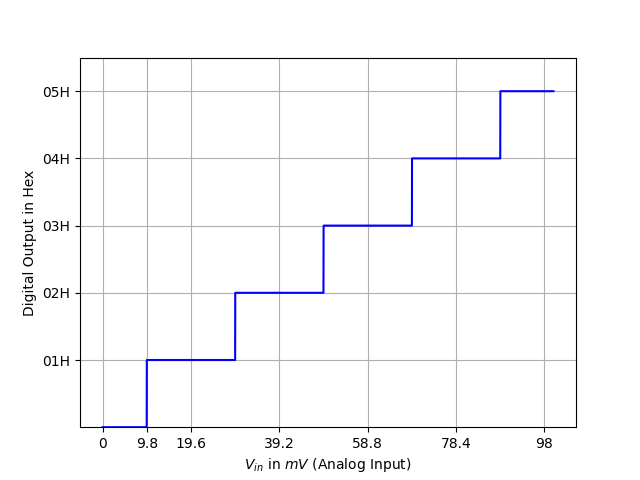
\includegraphics[width=\columnwidth]{2023/EE/40/figs/assign3.png}
    \caption{}
    \label{fig:ADC_plot_gate.ee.23.40}
\end{figure}

\newpage
\item Let x1\brak{t} and x2\brak{t} be two band-limited signals having bandwidth B = $4\pi\times10^3$
rad/s each. In the figure below, the Nyquist sampling frequency, in
rad/s, required to sample y\brak{t}, is
 \begin{circuitikz}
     \draw (0,0) node[left] {$x_1(t)$} to (0.8,0);
     \draw (0,-1) node[left] {$x_2(t)$} to (0.8,-1);
     \draw (1,0) circle(0.2);
     \draw (1,0) node {$\times$};
     \draw (1,-1) circle(0.2);
     \draw (1,-1) node {$\times$};
    \draw (1.2,0) to (1.8,0);
    \draw (1.2,-1) to (1.8,-1);
    \draw (1.8,0) to (1.8,-0.3);
    \draw (1.8,-1) to (1.8,-0.7);
    \draw (1.8,-0.5) circle(0.2);
    \draw (1.8,-0.5) node {$+$};
    \draw[->] (1,0.5) to (1,0.2) ;
    \node at (1,0.6) {cos$(4\pi\times10^3t)$};
    \draw[->] (1,-1.5) to (1,-1.2);
    \node at (1,-1.6) {cos$(12\pi\times10^3t)$};
    \draw (2,-0.5) to (2.3,-0.5);
    \node at (2.6,-0.5) {y(t)};
     
     
\end{circuitikz}
 \\
 \begin{enumerate}[label=(\alph*)]
    \item $20\pi\times10^3$
    \item $40\pi\times10^3$
    \item $8\pi\times10^3$
    \item $32\pi\times10^3$
\end{enumerate} \hfill(GATE EC 50)


\solution
\newpage


\end{enumerate}
